\section{Object definitions and Event selection}

\subsection{High Level Trigger Selection}


\begin{table}[h]
\centering
\caption{List of datasets used in the analysis.}
\begin{tabular}{|l|l|l|}
\hline
Year & Dataset & HLT                \\ \hline
2016 & SingleMuon     & HLT\_TkMu50 \\
     &                & HLT\_Mu50   \\
     & SingleElectron & HLT\_Ele27\_WPTight\_Gsf  \\
     & SinglePhoton   & HLT\_Photon175            \\ \hline
2017 & SingleMuon     & HLT\_Mu50       \\
     &                & HLT\_OldMu100   \\
     &                & HLT\_TkMu100    \\
     & SingleElectron & HLT\_Ele35\_WPTight\_Gsf  \\
     & SinglePhoton   & HLT\_Photon200            \\ \hline
2018 & SingleMuon & HLT\_Mu50     \\
     &            & HLT\_OldMu100 \\
     &            & HLT\_TkMu100  \\ \hline
     & EGamma     & HLT\_Ele32\_WPTight\_Gsf \\
     &            & HLT\_Photon200           \\ \hline
\end{tabular}
\label{tab:Datasets}
\end{table}




\begin{figure}[tph]
  \centering
        \subfigure[2016]{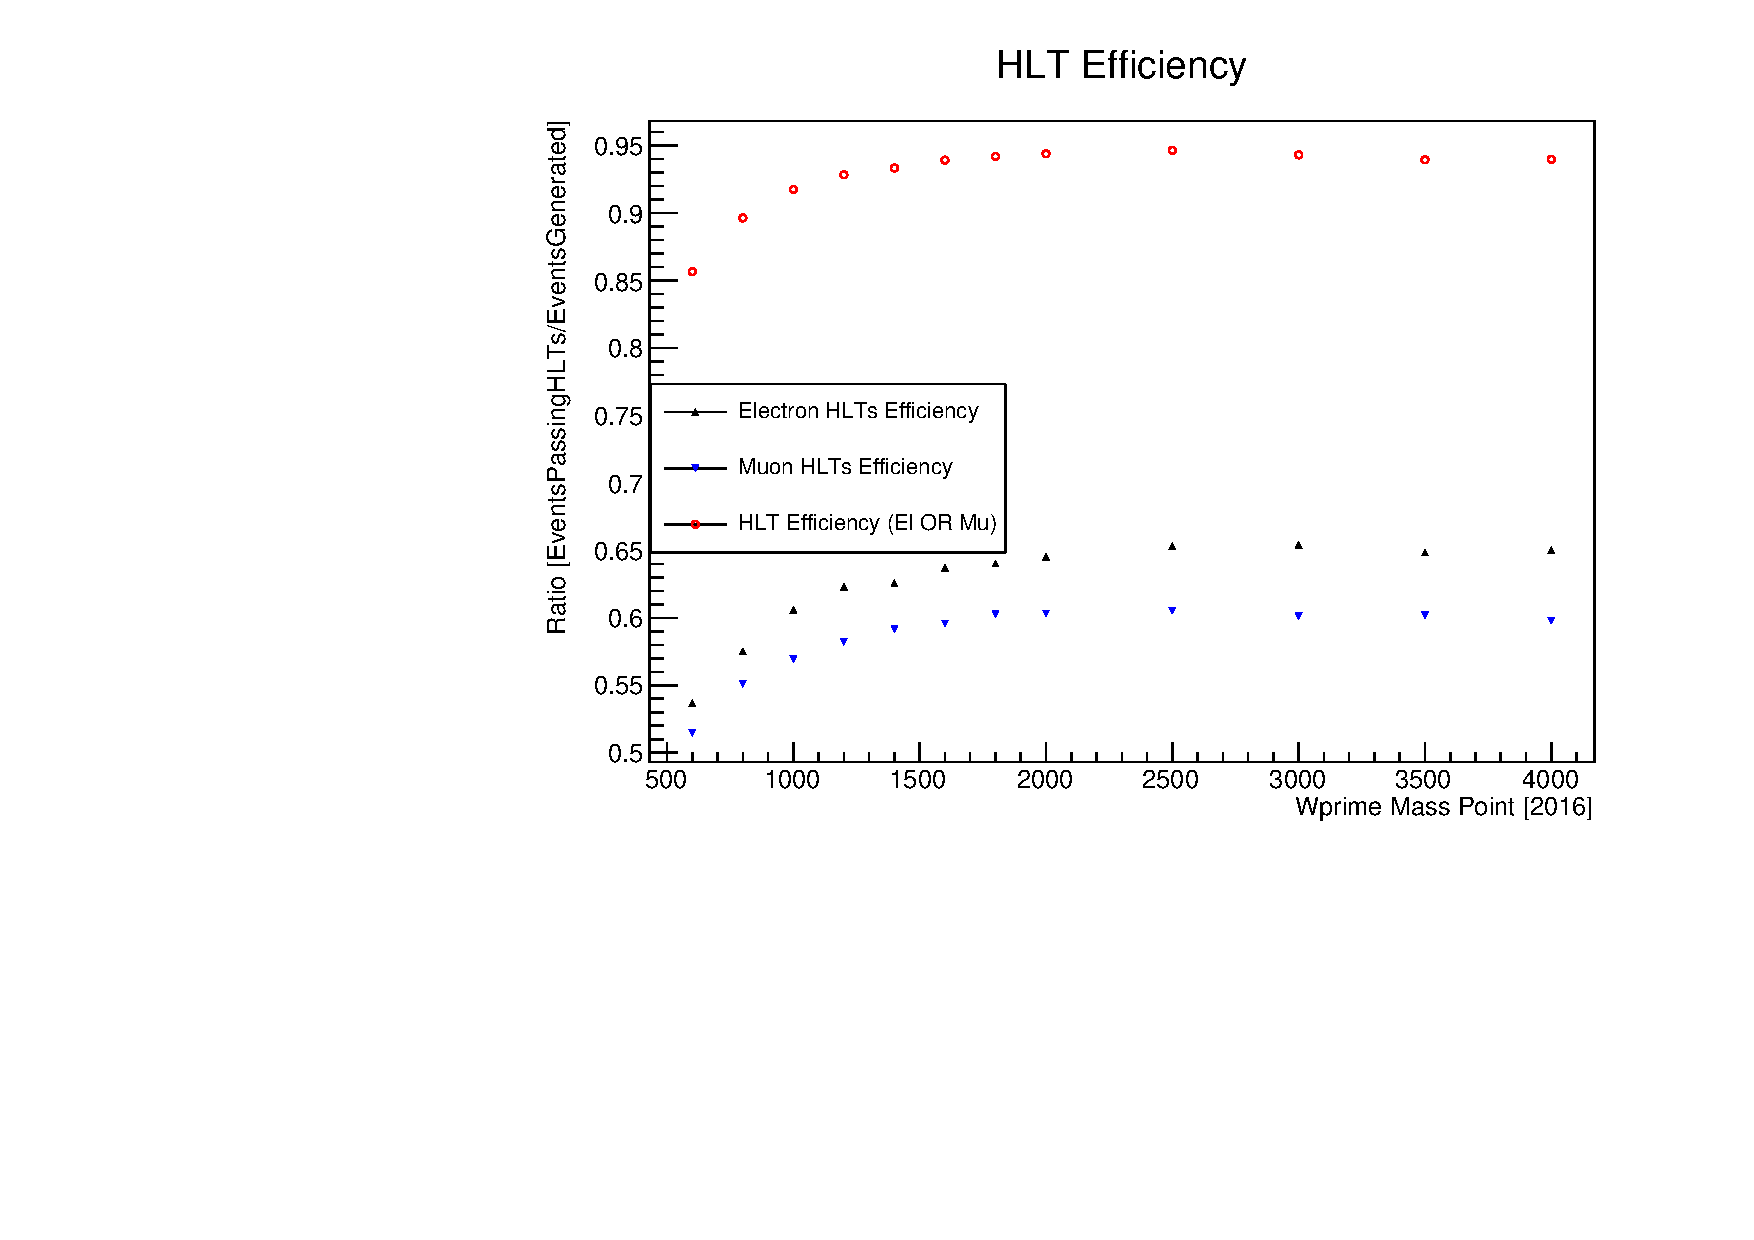
\includegraphics[width=.28\textwidth]{fig/2016_SignalTriggerEfficiency.pdf}}
        \subfigure[2017]{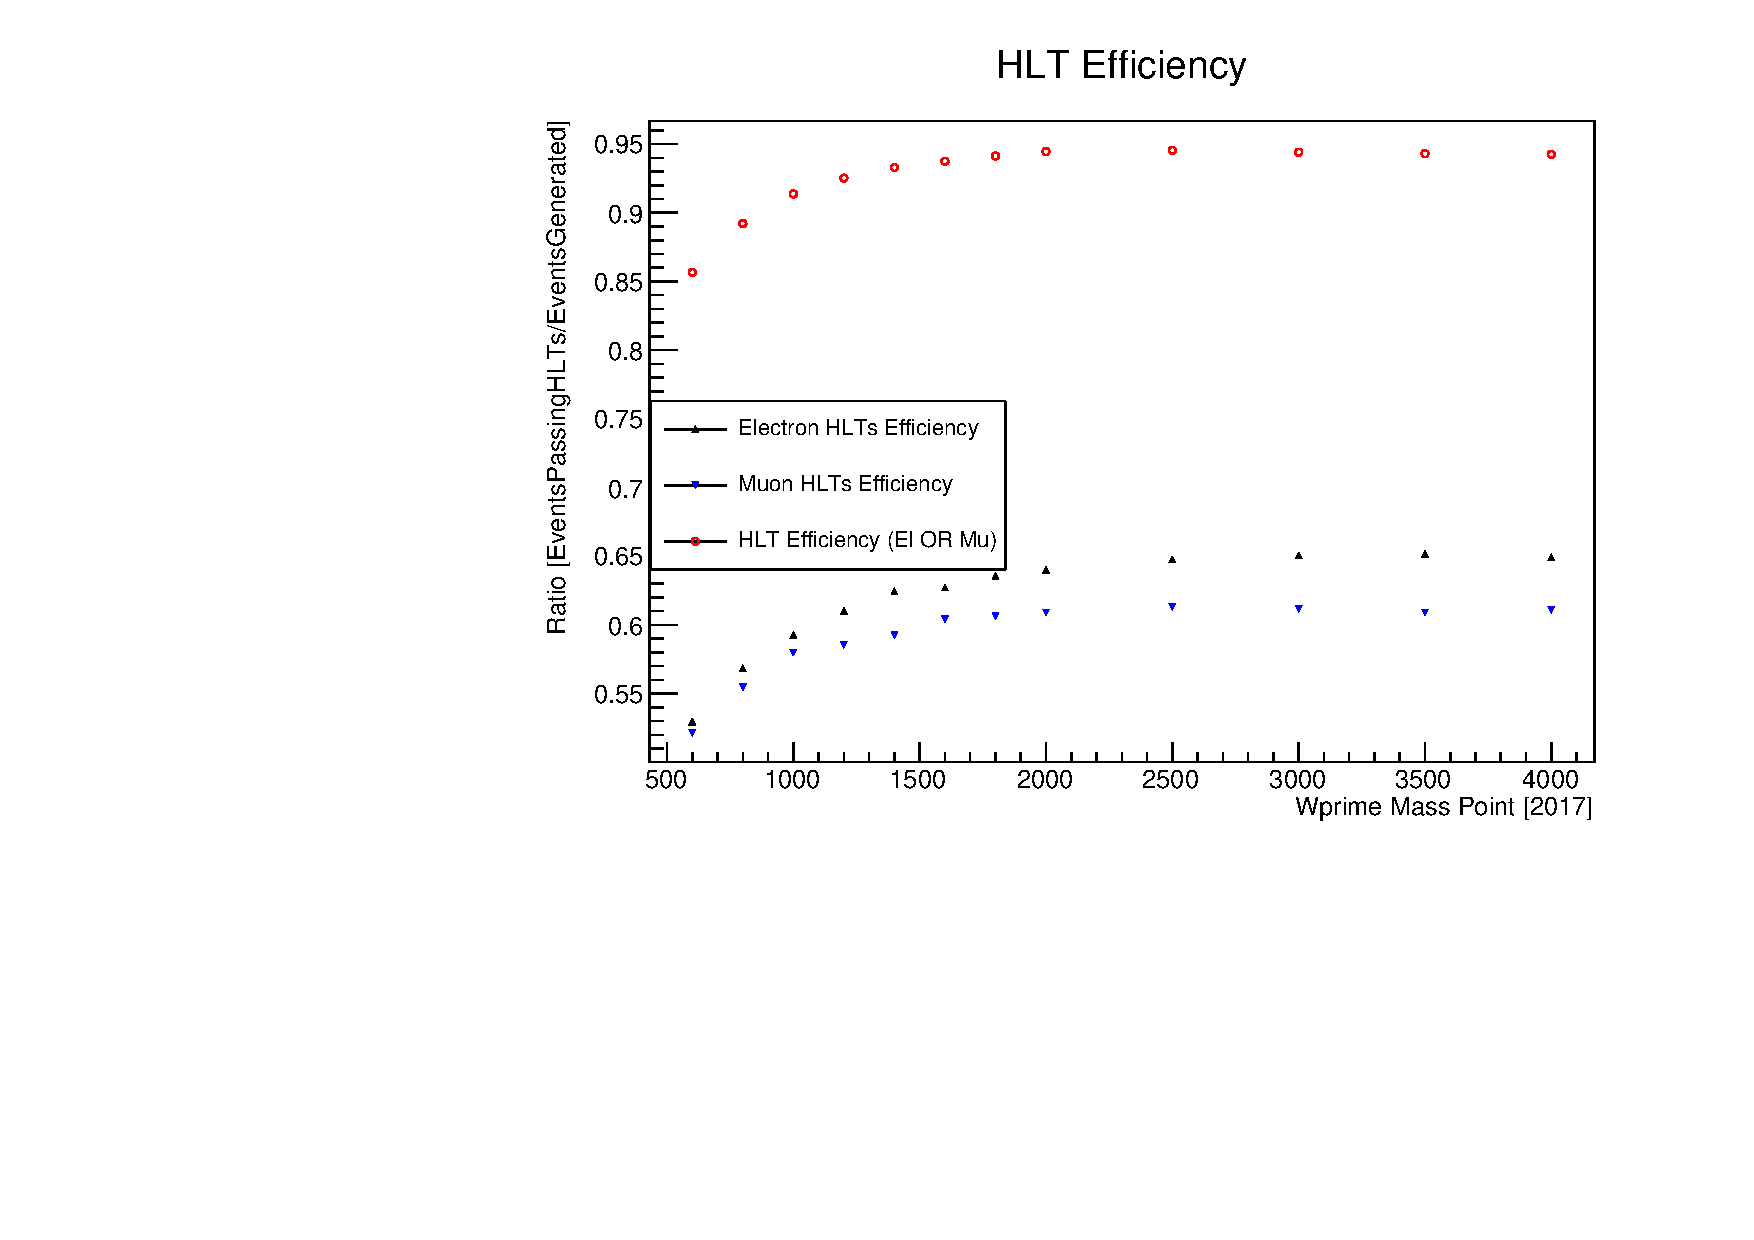
\includegraphics[width=.28\textwidth]{fig/2017_SignalTriggerEfficiency.pdf}}
        \subfigure[2018]{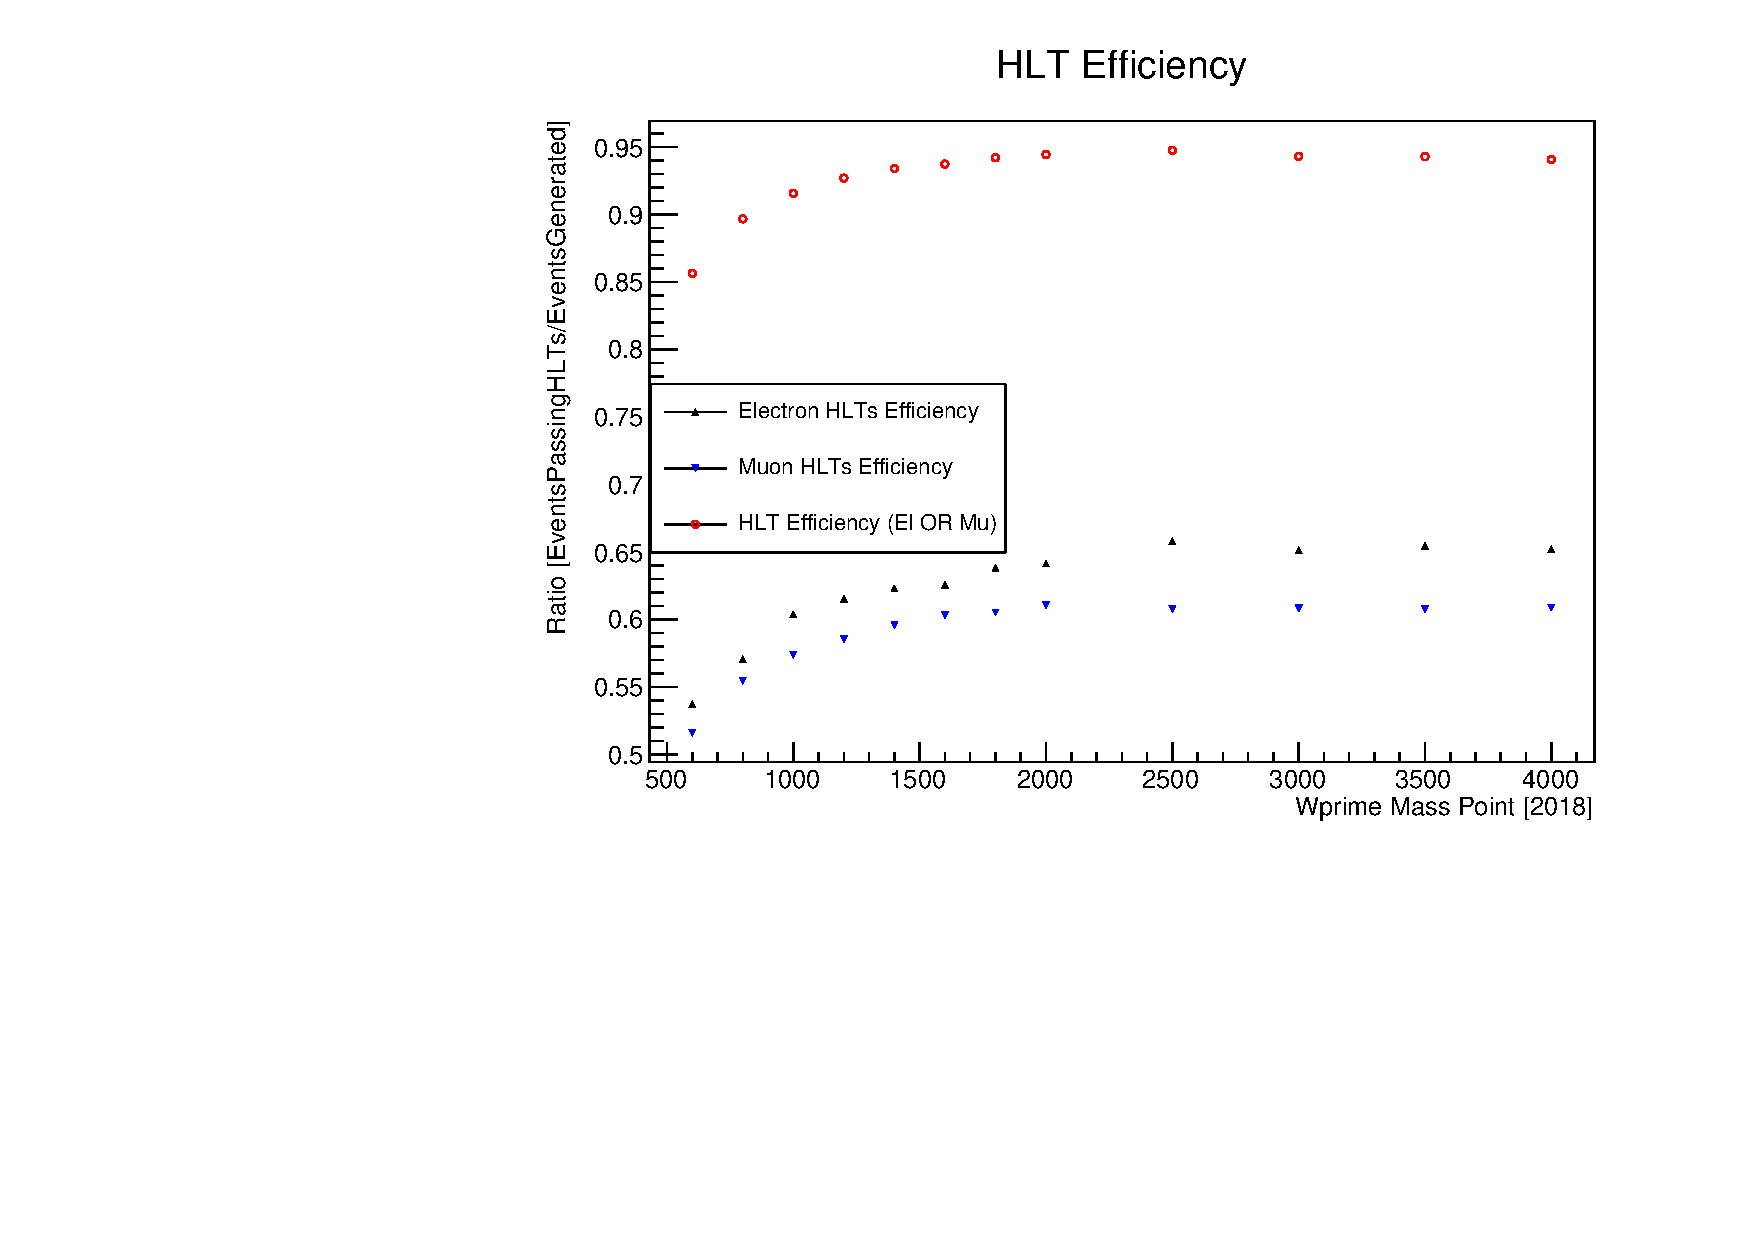
\includegraphics[width=.28\textwidth]{fig/2018_SignalTriggerEfficiency.pdf}}
  \caption{Signal efficiency for individual and combined High Level Triggers for Run II}
  \label{fig:hltSignalEfficiency}
\end{figure}

